%  BouMaton, a program to compute transformations on pictures.
%  Copyright (C) 2019  Frédéric Boulanger (frederic.boulanger@centralesupelec.fr)
% 
%  This program is free software: you can redistribute it and/or modify
%  it under the terms of the GNU General Public License as published by
%  the Free Software Foundation, either version 3 of the License, or
%  (at your option) any later version.
% 
%  This program is distributed in the hope that it will be useful,
%  but WITHOUT ANY WARRANTY; without even the implied warranty of
%  MERCHANTABILITY or FITNESS FOR A PARTICULAR PURPOSE.  See the
%  GNU General Public License for more details.
% 
%  You should have received a copy of the GNU General Public License
%  along with this program.  If not, see <https://www.gnu.org/licenses/>.
% © Frédéric Boulanger 1997-2019
\documentclass[a4paper]{article}
\usepackage[T1]{fontenc}
\usepackage[utf8]{inputenc}
\usepackage{ifthen}
\usepackage{xspace}
\usepackage{overpic}
\usepackage{mathptmx}
\usepackage[scaled=0.9]{helvet}
\usepackage{courier}
%\usepackage{garamath}
%\usepackage{gillsans}
\usepackage[francais]{babel}
\usepackage{sectsty}
\allsectionsfont{\sffamily\bfseries}
% Numéro de section dans la marge
\makeatletter
\def\@seccntformat#1{%
  \protect\makebox[0pt][r]{%
    \csname the#1\endcsname\quad
  }%
}
\makeatother

\usepackage[nohead,top=1cm,left=2.5cm,right=2cm,bottom=1.5cm,footskip=1cm]{geometry}
\usepackage{fancyhdr}
\pagestyle{fancy}
\fancyhead{}
\renewcommand{\headrulewidth}{0pt}
\lfoot{\textsf{\footnotesize BouMaton <\href{https://wdi.supelec.fr/boulanger/Software/}{wdi.supelec.fr/boulanger/Software/}>}}
\cfoot{\thepage}
\rfoot{\textsf{\footnotesize
  \href{mailto:frederic.boulanger@centralesupelec.fr}{<frederic.boulanger@centralesupelec.fr>}%
}}
\renewcommand{\footrulewidth}{0pt}

\usepackage[%
  pdfauthor={Frédéric Boulanger},
  pdftitle={Manuel de BouMaton},
  pdffitwindow,
  pdfstartview=XYZ,
  pdfpagemode=None
]{hyperref}

\newcommand{\signature}{%
  \vfill
  \begin{flushright}
    \href{mailto:Frederic.Boulanger@supelec.fr}{Frédéric Boulanger},
    \the\year-\ifnum\the\month<10 0\fi\the\month-\ifnum\the\day<10 0\fi\the\day
  \end{flushright}
}
\AtEndDocument{\signature}

%\setlength{\parindent}{0pt}
%\setlength{\parskip}{1ex plus 0.5ex minus 0.5ex}

\newcommand{\bouVersion}{2.0\xspace}
\newcommand{\bouRelease}{2019-04-24\xspace}

\newcommand{\BouMaton}{\textsf{BouMaton}\xspace}
\newcommand{\filename}[1]{\textsf{#1}}
\newcommand{\menu}[1]{\textsf{\textbf{#1}}}
\newcommand{\picdim}[2]{#1\,\(\times\)\,#2}

\begin{document}
  \begin{center}
    \textsf{\textbf{\large BouMaton v\bouVersion, \bouRelease}}
    
    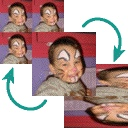
\includegraphics[scale=0.5]{icone}
    
    \href{mailto:Frederic.Boulanger@centralesupelec.fr}{\textsf{Frédéric Boulanger}}
  \end{center}
  
  
  \section{Qu'est-ce ?}
  \BouMaton est une application qui calcule deux transformations 
  d'images :
  \begin{itemize}
    \item la transformation du \textbf{photomaton} qui répartit les 
    pixels de l'image vers ses quatre coins, donnant ainsi un résultat 
    qui semble contenir quatre sous-images identiques à l'original, 
    comme dans un photomaton ;
    
    \item la transformation du \textbf{boulanger} qui étire une image 
    horizontalement avant de la replier afin qu'elle conserve sa taille 
    d'origine. Cette manœuvre est similaire au geste du boulanger qui 
    pétrit sa pâte, d'où le nom.
  \end{itemize}
  
  Ces deux transformations conservent toute l'information présente 
  dans l'image, il est donc toujours possible de retrouver l'original 
  en appliquant les transformations inverses. De plus, ces 
  transformations sont périodiques : après un certain nombre 
  d'itérations, on retrouve l'image d'origine.
  
  \BouMaton peut appliquer ces transformations et leurs inverses un 
  nombre quelconque de fois. Il calcule la période des transformations 
  pour l'image choisie, et conserve un historique des transformations 
  appliquées. Il peut aussi enregistrer le résultat des transformations 
  aux formats JPEG et PNG.
    
  \section{Pour démarrer}
  \BouMaton est une application Java. Sur la plupart des systèmes
  avec interface graphique, il suffit de double-cliquer le fichier
  \filename{BouMaton.jar} pour la lancer. Dans un terminal en ligne de
  commande, tapez \verb|java -jar BouMaton.jar| pour lancer \BouMaton.
  Sous Mac~OS~X, utilisez plutôt l'application \filename{BouMaton}
  (mais le fichier \filename{BouMaton.jar} ou la ligne de commande
  fonctionnent aussi).
  
  Lorsque \BouMaton est lancé, choisissez l'article \menu{Ouvrir...} du 
  menu \menu{Fichier} pour choisir une image. Les formats reconnus sont 
  ceux supportés par Java~1.4 : jpeg, gif et png.
  
  Cliquez sur l'un des boutons \menu{boulanger} ou \menu{photomaton}, 
  ou sélectionnez l'article correspondant dans le menu 
  \menu{Transformations} pour appliquer une transformation à l'image 
  affichée. Vous pouvez indiquer le nombre d'itérations de la 
  transformation (négatif pour obtenir la transformation inverse) dans 
  le champ de saisie situé entre les deux boutons.
  
  Si vous avez lancé le calcul d'un grand nombre d'itérations d'une 
  transformation sur une image de grande taille et trouvez que cela 
  prend trop de temps, vous pouvez interrompre le calcul grâce à 
  l'article \menu{Interrompre} du menu \menu{Transformations}.
  
  \section{Une description plus détaillée}
  La fenêtre principale de \BouMaton contient les éléments suivants :
  \begin{center}
    \sffamily
    \begin{overpic}[%
                    scale=.4,
                    %grid
                   ]{vue_generale_fr}
      \put(-10,80){\makebox(0,0)[br]{zone d'affichage}}
      \put(-10,80){\vector(2,-1){25}}
      %
      \put(-10,20){\makebox(0,0)[br]{avancement du calcul de la période}}
      \put(-10,20){\vector(3,-1){12}}
      %
      \put(-10,12){\makebox(0,0)[br]{transformation du boulanger}}
      \put(-10,12){\vector(4,-1){12}}
      %
      \put(20,-2){\makebox(0,0)[tr]{dimensions de l'image}}
      \put(20,-2){\vector(1,2){8}}
      %
      \put(36,-2){\makebox(0,0)[tl]{nombre d'itérations}}
      \put(35,-2){\vector(0,1){8}}
      %
      \put(80,12){\makebox(0,0)[bl]{transformation du photomaton}}
      \put(80,12){\vector(-4,-1){10}}
      %
      \put(80,20){\makebox(0,0)[bl]{période de la transformation du photomaton}}
      \put(80,20){\vector(-3,-1){17}}
    \end{overpic}
  \end{center}

  \vspace{2cm}
  
  La zone d'affichage montre le résultat de l'application des 
  transformations à l'image. La barre d'avancement du calcul de la 
  période indique que la période de la transformation du boulanger pour 
  cette image est en cours de calcul. Quand le calcul sera terminé, la 
  barre d'avancement sera remplacée par le résultat.

  Les boutons \menu{boulanger} et \menu{photomaton} provoquent le 
  calcul de la transformation correspondante, appliquée autant de fois 
  qu'indiqué dans le champ de saisie.

  Sur la droite, vous pouvez voir la période de la transformation du 
  photomaton pour cette image (elle est beaucoup plus rapide à calculer 
  que celle de la transformation du boulanger).

  Dans l'exemple suivant, la zone d'affichage montre le résultat de la 
  transformation du photomaton appliquée à l'image de départ, et le 
  programme est en train de calculer 500 itérations de la 
  transformation du photomaton :
  \begin{center}
    \sffamily
    \begin{overpic}[%
                    scale=.4,
                    %grid
                   ]{photomaton}
      \put(-10,12){\makebox(0,0)[br]{%
        \parbox{70\unitlength}{%
          désactivé car une transformation est en cours de calcul
        }%
      }}
      \put(-10,12){\vector(4,-1){12}}
      %
      \put(30,-17){\makebox(0,0)[t]{nous voulons 500 itérations}}
      \put(30,-15){\vector(1,4){5}}
      %
      \put(80,12){\makebox(0,0)[bl]{%
        \parbox{70\unitlength}{%
          désactivé car une transformation est en cours de calcul
        }%
      }}
      \put(80,15){\vector(-4,-1){17}}
      %
      \put(80,0){\makebox(0,0)[tl]{%
        \parbox{70\unitlength}{%
          avancement du calcul des 500 itérations de la transformation du 
          photomaton
        }%
      }}
      \put(80,0){\vector(-4,1){14}}
    \end{overpic}
  \end{center}
  
  \vspace{2cm}
  
  Pour la transformation du boulanger, le comportement est similaire : 
  dans l'exemple suivant, le résultat de la transformation du boulanger 
  appliquée à l'image de départ est affiché, et le programme est en 
  train de calculer 500 itérations de la transformation du boulanger :
  \begin{center}
    \sffamily
    \begin{overpic}[%
                    scale=.4,
                    %grid
                   ]{boulanger}
      \put(-10,12){\makebox(0,0)[br]{%
        \parbox{70\unitlength}{%
          désactivé car une transformation est en cours de calcul
        }%
      }}
      \put(-10,12){\vector(4,-1){12}}
      %
      \put(30,-17){\makebox(0,0)[t]{nous voulons 500 itérations}}
      \put(30,-15){\vector(1,4){5}}
      %
      \put(80,12){\makebox(0,0)[bl]{%
        \parbox{70\unitlength}{%
          désactivé car une transformation est en cours de calcul
        }%
      }}
      \put(80,15){\vector(-4,-1){17}}
      %
      \put(-10,0){\makebox(0,0)[tr]{%
        \parbox{70\unitlength}{%
          avancement du calcul des 500 itérations de la transformation du 
          boulanger
        }%
      }}
      \put(-10,0){\vector(4,1){10}}
    \end{overpic}
  \end{center}
  
  \vspace{2cm}

  \section{Enregistrement des images}
	\BouMaton est capable d'enregistrer les images aux formats JPEG et PNG.

  Le format JPEG donne des fichiers plus petits pour les
  photographies, mais il supprime des détails qui sont considérés
  comme mineurs lorsqu'on prend en compte la manière dont un être
  humain voit.  Lorsqu'on enregistre une image au format JPEG, on peut
  choisir la quantité d'information qui sera perdue en ajustant la
  qualité de l'image enregistrée.Le réglage varie de 0 (forte
  compression, fichier de petite taille, mais qualité très faible), à
  100 (compression faible, fichier de plus grande taille, mais
  meilleure qualité).  Pour vous aider dans votre choix, \BouMaton
  peut calculer une estimation de la taille qu'aurait le fichier avec
  le réglage courant si vous cliquez le bouton \menu{Calculer la
  taille} de ce dialogue.  Si la taille estimée est plus petite que la
  taille du fichier JPEG d'origine, votre réglage est sûrement trop
  faible.  Si elle est beaucoup plus élevée, votre réglage est
  sûrement trop fort.  Comme les transformations rendent l'image de
  plus en plus complexe, il est normal que la taille estimée croisse
  pour les résultats de transformations successives, à réglage de
  qualité JPEG constant.
  
  Le format PNG n'élimine aucune information et fournit donc
  généralement des fichiers beaucoup plus gros que le format JPEG. 
  Toutefois, ce format utilise un algorithme de compression sans 
  perte qui est plus efficace que la compression JPEG sur les images 
  qui ne contiennent que des lignes et des zones de couleur uniforme. 
  Comme le format PNG ne supprime pas d'information, vous pouvez 
  l'utiliser pour enregistrer des images transformées dont vous 
  souhaitez restaurer plus tard l'aspect d'origine en appliquant les 
  transformations inverses.
    
%   \section{Enregistrement des images en JPEG}
%   Si \BouMaton a trouvé les classes nécessaires sur votre
%   ordinateur, l'article \menu{Enregistrer...} du menu \menu{Fichier}
%   est accessible et vous permet d'enregistrer les merveilleuses images
%   que vous obtiendrez avec \BouMaton. Le seul format de fichier
%   supporté pour l'enregistrement est le JPEG. Ce format réduit la
%   taille du fichier contenant une image en ignorant les détails qu'il
%   considère comme moins important à cause de la manière dont l'œil
%   humain voit. Quand vous enregistrer une image dans un fichier,
%   \BouMaton affiche un dialogue vous permettant de déterminer la
%   quantité d'information à préserver lors de la compression JPEG.
%   Le réglage varie de 0 (forte compression, fichier de petite taille,
%   mais qualité très faible), à 100 (compression faible, fichier de
%   plus grande taille, mais meilleure qualité). Pour vous aider dans
%   votre choix, \BouMaton peut calculer une estimation de la taille
%   qu'aurait le fichier avec le réglage courant si vous cliquez le
%   bouton \menu{Calculer la taille} de ce dialogue. Si la taille
%   estimée est plus petite que la taille du fichier JPEG d'origine,
%   votre réglage est sûrement trop faible. Si elle est beaucoup plus
%   élevée, votre réglage est sûrement trop fort. Comme les
%   transformations rendent l'image de plus en plus complexe, il est
%   normal que la taille estimée croisse pour les résultats de
%   transformations successives, à réglage de qualité JPEG constant.
  
  \section{Historique des transformations}
  \BouMaton conserve la trace des transformations appliquées à une 
  image depuis son chargement. Vous pouvez afficher cet historique 
  grâce à l'article \menu{Afficher l'historique} du menu 
  \menu{Transformations} :
  \begin{center}
    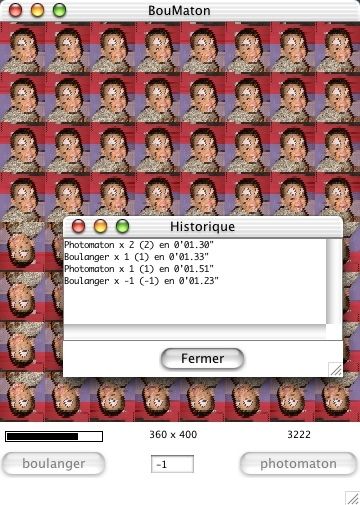
\includegraphics[scale=0.4]{history_fr}
  \end{center}
  Les transformations successives identiques sont fusionnées dans 
  l'historique, de sorte que deux transformations du photomaton 
  successives donneront une seule entrée (avec un nombre d'itérations 
  égal à 2) dans l'historique. Chaque entrée donne la nature de la 
  transformation, le nombre d'itérations demandées, le nombre 
  d'itérations effectivement calculées, et le temps mis pour effectuer 
  le calcul. Le nombre d'itérations effectivement calculées peut être 
  inférieur au nombre d'itérations demandées, car calculer 3225 
  itérations d'une transformation dont la période est 3222 revient 
  exactement au même que calculer seulement 3 itérations, ce qui prend 
  beaucoup moins de temps. Avec la même période, si vous demandez 3200 
  itérations, \BouMaton calculera 22 itérations de la transformation 
  inverse puisque c'est plus rapide.

  Vous pouvez toujours revenir à l'image d'origine grâce à l'article 
  \menu{Restaurer l'original} du menu \menu{Fichier}. Cela efface 
  aussi l'historique des transformations.
  
  \section{Informations sur les transformations}
  Lorsqu'il calcule la période des transformations, \BouMaton collecte 
  des informations sur la période de chaque pixel de l'image. Au cours 
  de transformations successives, chaque pixel parcourt une orbite (il 
  passe par une suite de positions successives) et peut revenir à sa 
  position initiale bien avant que toute l'image retrouve sa forme 
  initiale. La période de la transformation est le plus petit nombre 
  d'itérations tel que tous les pixels de l'image ont fait un nombre 
  entier de tours sur leur orbite.
  
  Il peut arriver qu'après un certain nombre d'itérations, un grand 
  nombre de pixels soient revenus à leur position initiale, sans 
  qu'ils le soient tous. L'image de départ semble alors émerger d'une 
  sorte de brouillard aléatoire de pixels.

  En choisissant l'article \menu{Afficher les informations} du menu 
  \menu{Transformations}, vous affichez les informations collectées 
  sur les deux transformations. Les informations concernant la 
  transformation du boulanger sont assez longues à calculer et 
  n'apparaissent que lorsque la période de cette transformation est 
  calculée.
  
  \begin{center}
    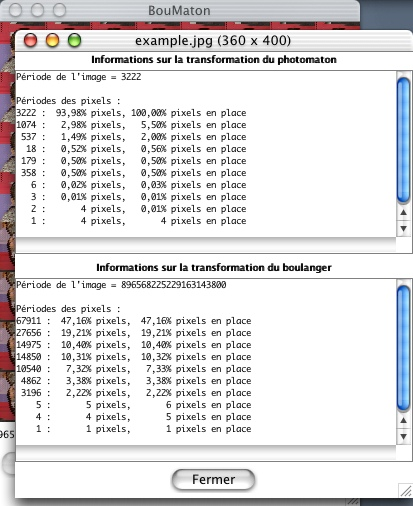
\includegraphics[scale=0.4]{info_exemple_fr}
  \end{center}
  Cet exemple montre les informations obtenues pour une image de 
  \picdim{360}{400} pixels (les périodes ne dépendent que de la 
  géométrie de l'image, pas de son contenu). On peut voir que la 
  période de la transformation du boulanger est vraiment grande, mais 
  qu'après 67911 itérations, 47,16\,\% des pixels ont retrouvé leur 
  position initiale.
  
  \section{Exemples}
  Les suites d'images suivantes montrent l'évolution d'une image pour 
  chacune des transformations. Partant de l'original, on passe 
  ensuite à des images où toute information semble perdue, ainsi qu'à 
  d'autres où des motifs fantômes apparaissent, pour finalement 
  revenir à l'image d'origine.
  
  \subsection{Itérations de la transformation du photomaton}

  {\sffamily\small
  \begin{tabular}{@{}*5{p{0.18\textwidth}}@{}}
    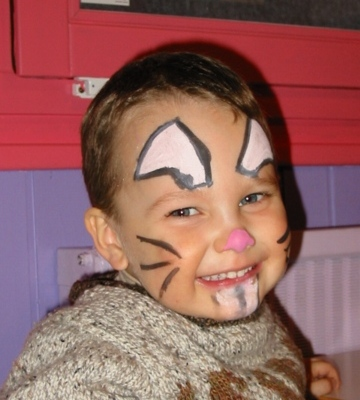
\includegraphics[width=\linewidth]{example}
    &
    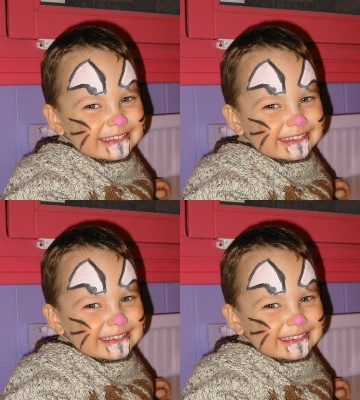
\includegraphics[width=\linewidth]{example_p1}
    &
    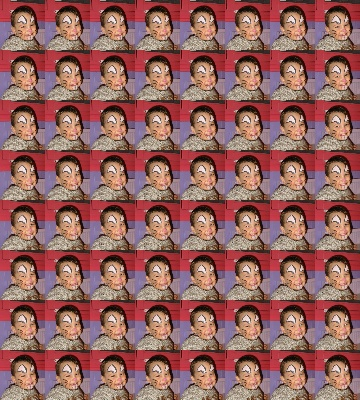
\includegraphics[width=\linewidth]{example_p3}
    &
    
\includegraphics[width=\linewidth]{example_p8}
    &
    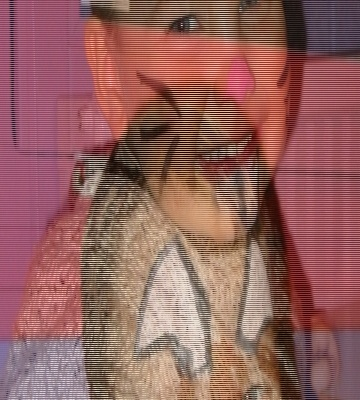
\includegraphics[width=\linewidth]{example_p179}
    \\
      image d'origine
    & après une itération
    & après 3 itérations
    & après 8 itérations
    & quelque chose apparaît après 179 itérations
    \\[10pt]
    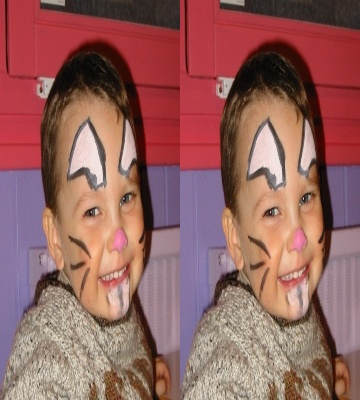
\includegraphics[width=\linewidth]{example_p180}
    &
    
\includegraphics[width=\linewidth]{example_p_6}
    &
    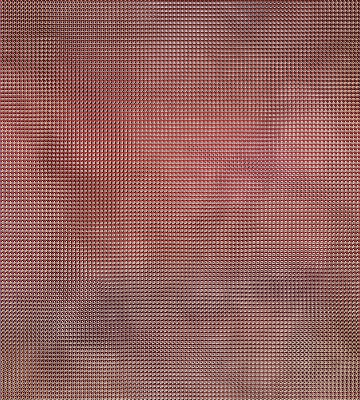
\includegraphics[width=\linewidth]{example_p_2}
    &
    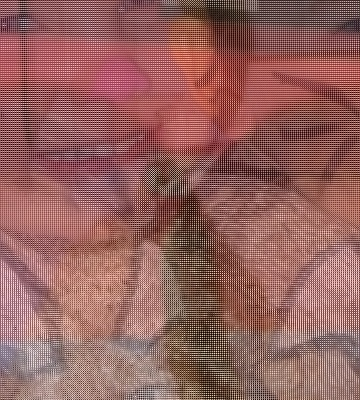
\includegraphics[width=\linewidth]{example_p_1}
    &
    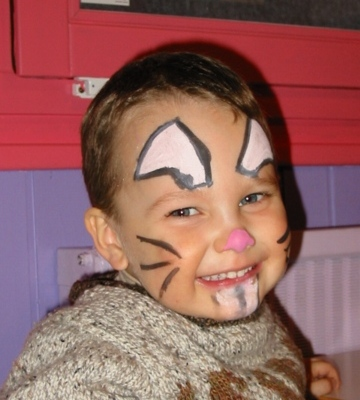
\includegraphics[width=\linewidth]{example}
    \\
      on est près de l'original après 180 itérations
    & 6 itérations avant le retour à l'original
    & 2 itérations avant le retour à l'original
    & 1 itération avant le retour à l'original
    & retour à l'original après 3222 itérations
  \end{tabular}
  }
  
  \subsection{Itérations de la transformation du boulanger}
  {\sffamily\small
  \begin{tabular}{@{}*5{p{0.18\textwidth}}@{}}
    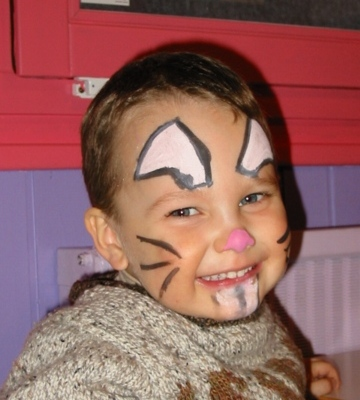
\includegraphics[width=\linewidth]{example}
    &
    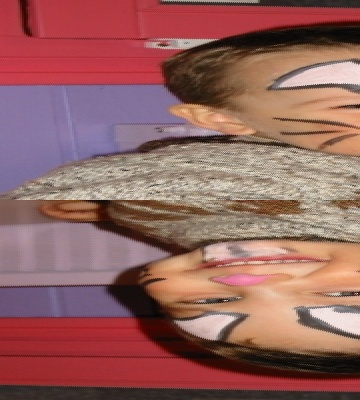
\includegraphics[width=\linewidth]{example_b1}
    &
    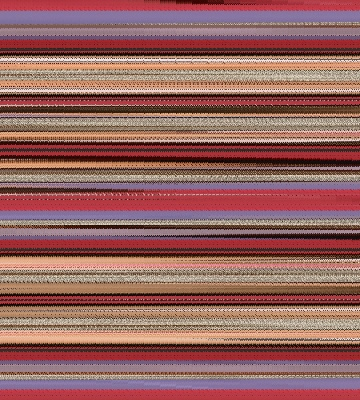
\includegraphics[width=\linewidth]{example_b4}
    &
    
\includegraphics[width=\linewidth]{example_b20}
    &
    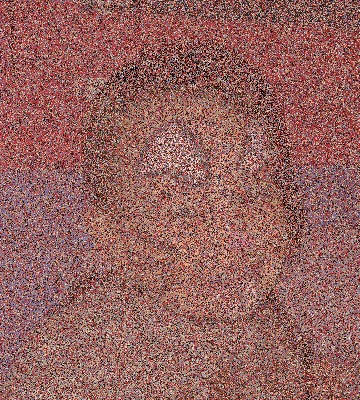
\includegraphics[width=\linewidth]{example_b27656}
    \\
      image d'origine
    & après une itération
    & après 4 itérations
    & après 20 itérations
    & 19,2\% des pixels sont en place après 27656 itérations
    \\[10pt]
    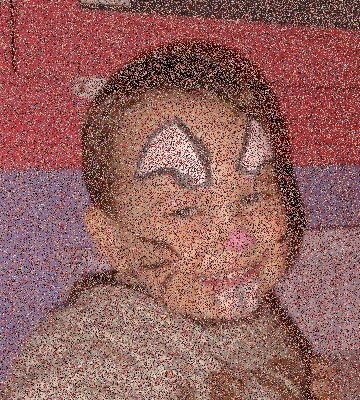
\includegraphics[width=\linewidth]{example_b67911}
    &
    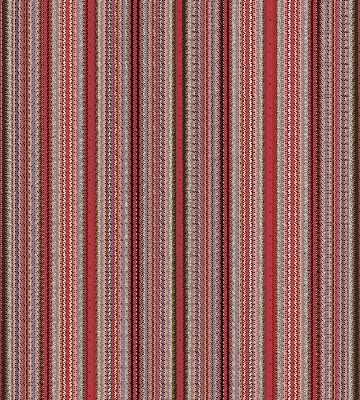
\includegraphics[width=\linewidth]{example_b_6}
    &
    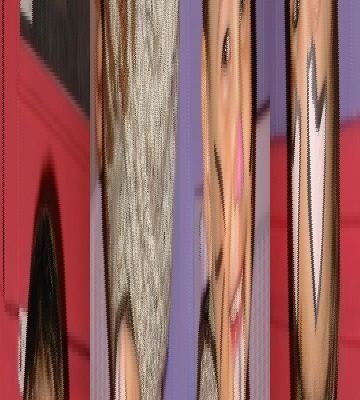
\includegraphics[width=\linewidth]{example_b_2}
    &
    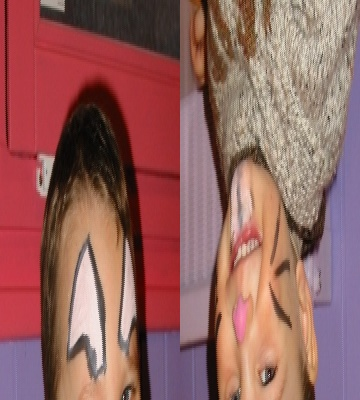
\includegraphics[width=\linewidth]{example_b_1}
    &
    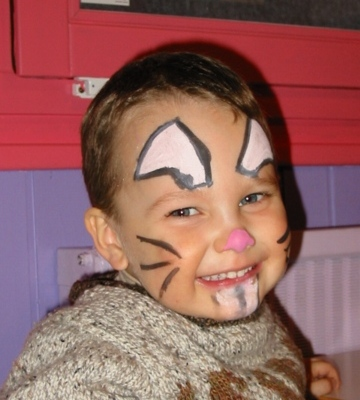
\includegraphics[width=\linewidth]{example}
    \\
      47.2\% des pixels sont en place après 67911 itérations
    & 6 itérations avant le retour à l'original
    & 2 itérations avant le retour à l'original
    & 1 itération avant le retour à l'original
    & retour à l'original après {\tiny 896568225229163143800} itérations
  \end{tabular}
  }
  
  \section{Licence}
  \newlength{\savedindent}
  \setlength{\savedindent}{\parindent}
  \setlength{\parindent}{0pt}
  \newlength{\savedskip}
  \setlength{\savedskip}{\parskip}
  \setlength{\parskip}{1ex}
  
  \BouMaton est Copyright © Frédéric Boulanger 1997-2019.
  
  Ce programme est un logiciel libre ; vous pouvez le redistribuer ou le modifier
  suivant les termes de la GNU General Public License telle que publiée par la
  Free Software Foundation. Vous pouvez utiliser soit la version 3 de la licence, 
  soit, à votre gré, toute version ultérieure.
  
  Ce programme est distribué dans l'espoir qu'il sera utile, mais sans aucune garantie, 
  y compris la garantie implicite de qualité marchande ou d'adéquation à un objectif
  particulier. Consultez la GNU General Public License pour plus de détails.
  
  Une copie de cette licence vous est fournie avec ce programme, si ce n'est pas le cas, 
  consultez :
  \begin{center}
  	\url{http://www.gnu.org/licenses}
  \end{center}
  
  \setlength{\parindent}{\savedindent}
  \setlength{\parskip}{\savedskip}
  
  \section{L'histoire de \BouMaton}
  Tout a commencé avec un article de Jean-Paul Delahaye et Philippe
  Mathieu dans le numéro de décembre 1997 (242) de «~Pour la
  Science~».  Cet article présentait les transformations du
  boulanger et du photomaton, et j'ai alors commencé à coder ces
  transformations en C. Pour éviter d'avoir à écrire une
  application complète, j'ai utilisé le mécanisme de modules
  d'extension de GraphicConverter, une application pour
  Mac~OS qui est capable de lire et de créer presque n'importe quel
  type de fichier graphique
  (\url{http://www.bonnaure.com/GraphicConverter/info.html}). Cela 
  déboucha sur la création de deux modules d'extension nommés 
  \filename{PhotoMaton} et \filename{Boulanger}.

  GraphicConverter a évolué vers Carbon lorsque Mac~OS~X est sorti, et 
  au lieu de passer mes modules d'extension à Carbon, j'ai décidé 
  d'écrire une application Java combinant les fonctionnalités des deux 
  modules. Cela m'a permis de gérer l'historique des transformations 
  appliquées à une image et d'afficher les informations concernant la 
  période pour l'image complète ainsi que pour chacun de ses pixels. 
  En utilisant la classe BigInteger, j'ai pu corriger une erreur dans 
  le calcul de la période de la transformation du boulanger qui 
  provoque fréquemment des débordements arithmétiques lorsqu'on utilise 
  les \verb|unsigned long| de C.

  Le résultat est \BouMaton, et j'espère que les utilisateurs des 
  modules GraphicConverter l'apprécieront, et que les utilisateurs de 
  Windows ou d'Unix profiteront de la devise «~coder une fois, exécuter 
  partout~» de Java...
  
  \medskip
  
  \noindent La version 1.0 est la première version publique de \BouMaton.
  \par\smallskip
  \noindent La version 1.1 règle un problème de rafraîchissement des images.
  \par\smallskip
  \noindent La version 1.2 améliore la gestion des situations où la 
  mémoire vient à manquer, et ajoute un dialogue permettant de choisir 
  la qualité de la compression JPEG lors de l'enregistrement des images.
  \par\smallskip
  \noindent La version 1.3 utilise un nouvel algorithme pour calculer 
  la période de la transformation du boulanger beaucoup plus rapidement.
  \par\smallskip
  \noindent La version 1.4 utilise le package 
  \filename{javax.imageio} et permet d'enregistrer les images au 
  format PNG.
  \par\smallskip
  \noindent La version 1.5 résoud un problème de lecture des images PNG.
  \par\smallskip
  \noindent La version 2.0 est une mise à jour du code après 13 ans sans changement. 
  Il en existe une version pour Java 8 et une pour Java 11.
  
  \section{Détails techniques\label{sec:tech-details}}
  Cette section expose des détails techniques de \BouMaton et peut 
  être ignorée par les utilisateurs qui souhaitent simplement appliquer 
  des transformations à leurs images.
  
  \subsection{Traduire \BouMaton}
  Le manuel de \BouMaton est écrit en \LaTeX. Vous pouvez vous inspirer 
  de la version anglaise ou de la version française du manuel pour le 
  traduire en une autre langue. Vous devez alors indiquer que la 
  traduction est de vous.

  Les chaînes de caractères utilisées dans \BouMaton peuvent être 
  traduites en d'autres langues. Deux classes 
  \filename{BouMatonStrings.properties} et \filename{BouMatonStrings\_fr.properties} 
  contiennent respectivement les chaînes de caractères en anglais et en français. 
	Le fichier \filename{BouMatonStrings\_fr.properties} est utilisé quand la 
  locale par défaut indique que la langue est le français, sinon, c'est 
  \filename{BouMatonStrings.properties} qui est utilisé. Si vous 
  souhaitez traduire \BouMaton en une autre langue, vous devez écrire 
  un fichier \filename{BouMatonStrings\_<lang>.java}, où 
  \filename{<lang>} est le code de cette langue pour la locale (par 
  exemple \filename{de} pour l'allemand, \filename{it} pour l'italien 
  etc). La manière la plus simple d'écrire ce fichier est de partir 
  d'une copie d'un des fichiers existants et de traduire chaque 
  expression située en second argument de \texttt{strings.put} sur chaque ligne.
  Le nouveau fichier doit être ajouté à l'archive jar une fois compilé pour que les 
  nouvelles chaînes de caractères soient utilisées lorsque la locale 
  correspondante est active.

  Si vous traduisez \BouMaton, merci de me faire parvenir les fichiers 
  correspondants afin que je les inclue dans les prochaines versions. 
  Si une traduction du manuel accompagne les fichiers, ce sera encore mieux.
  
  \subsection{La transformation du boulanger}
  L'étirement horizontal de l'image dans la transformation du boulanger 
  est obtenu en entrelaçant les pixels des lignes impaires avec ceux 
  des lignes paires. Le repliement consiste à couper l'image étirée à 
  la largeur de l'image de départ, puis à faire pivoter la partie 
  droite autour de son coin inférieur gauche, comme indiqué ci-dessous 
  pour une image \picdim{4}{4} :
  
  \begin{center}
    \newcommand{\pixbox}[2]{\makebox(1,1){\textsf{\scriptsize(#1,#2)}}}
    \newcounter{pixx}
    \newcounter{pixy}
    \newcounter{pixnum}
    \newcommand{\dopixbox}[2]{%
      \put(\thepixx,\thepixy){\pixbox{#1}{#2}}%
      \stepcounter{pixx}%
      \bouline{\thepixy}{\thepixx}{\thepixnum}%
    }
    \newcommand{\bouline}[3]{%
      \let\next=\relax
      \ifnum#2<#3
        \setcounter{pixy}{#1}%
        \setcounter{pixx}{#2}%
        \setcounter{pixnum}{#3}%
        \let\next=\dopixbox
      \fi
      \next
    }
    \setlength{\unitlength}{0.5cm}
    \begin{picture}(22,4)
      \put(0,0){\framebox(4,4){}}
      \multiput(0,1)(0,1){3}{\line(1,0){4}}
      \multiput(1,0)(1,0){3}{\line(0,1){4}}
      \bouline{3}{0}{4} 0 0  0 1  0 2  0 3
      \bouline{2}{0}{4} 1 0  1 1  1 2  1 3
      \bouline{1}{0}{4} 2 0  2 1  2 2  2 3
      \bouline{0}{0}{4} 3 0  3 1  3 2  3 3
      %%
      \put(5,2){\vector(1,0){1}}
      %%
      \qbezier(0.5,3.9)(6,5)(7.5,2.9)\put(7.5,2.9){\circle*{0.12}}
      \qbezier(0.5,2.1)(6,1)(8.5,2.1)\put(8.5,2.1){\circle*{0.12}}
      %%
      \put(7,1){\framebox(8,2){}}
      \put(7,2){\line(1,0){8}}
      \multiput(8,1)(1,0){7}{\line(0,1){2}}
      \bouline{2}{7}{15} 0 0  1 0  0 1  1 1  0 2  1 2  0 3  1 3
      \bouline{1}{7}{15} 2 0  3 0  2 1  3 1  2 2  3 2  2 3  3 3
      %%
      \put(16,2){\vector(1,0){1}}
      %%
      \put(11,1){\circle*{0.25}}
      \put(11,0.9){\oval(3.5,3)[br]}
      \put(11,-0.6){\vector(-1,0){0.5}}     
      %%
      \put(18,0){\framebox(4,4){}}
      \multiput(18,1)(0,1){3}{\line(1,0){4}}
      \multiput(19,0)(1,0){3}{\line(0,1){4}}
      \bouline{3}{18}{22} 0 0  1 0  0 1  1 1
      \bouline{2}{18}{22} 2 0  3 0  2 1  3 1
      \bouline{1}{18}{22} 3 3  2 3  3 2  2 2
      \bouline{0}{18}{22} 1 3  0 3  1 2  0 2
      %%
      \put(22,2){\circle*{0.25}}
      \put(22.2,2){\oval(3,3)[br]}\put(22.2,0.5){\vector(-1,0){0.1}}
    \end{picture}
  \end{center}

  Il n'y a aucune perte d'information au cours de cette transformation, 
  et après un certain nombre d'itérations, l'image de départ reparaît. 
  Toutefois, je ne connais pas de formule donnant cette période pour 
  n'importe quelle image. Pour une image de \(2^m\) par \(2^m\) pixels, 
  l'image de départ reparaît après \(2m+1\) itérations. Pour une image 
  de \(2^m\) par \(2^n\) pixels, il faut attendre \((2m+1)(2n+1)+1\) 
  itérations.

  Pour calculer la période de la transformation pour une image donnée, 
  \BouMaton calcule la période \(P(x,y)\) de chaque pixel de l'image 
  (le nombre d'itérations nécessaires pour qu'il reprenne sa position 
  initiale dans l'image). La période \(P\) pour l'image est le plus 
  petit multiple commun à toutes les périodes \(P(x,y)\) des pixels de 
  l'image. Ce calcul peut être assez long, et \BouMaton utilise un 
  flot de contrôle (thread) distinct pour le calculer, afin que l'on 
  puisse faire autre chose pendant qu'il s'exécute. La période de cette 
  transformation peut être très grande (896568225229163143800 pour une 
  image \picdim{360}{400}), et \BouMaton utilise la classe BigInteger 
  de Java pour calculer le PPCM des périodes des pixels.
  
  Depuis la version 1.3, \BouMaton utilise un nouvel algorithme pour 
  calculer cette période bien plus rapidement qu'avant. Lorsqu'on 
  calcule la période d'un pixel, on trouve tous les pixels qui 
  appartiennent à son orbite. Tous ces pixels ont la même période 
  puisqu'ils appartiennent à la même orbite, il n'est donc pas 
  nécessaire de calculer leur période ultérieurement. Comme il y a en 
  général peu d'orbites dans une image, le nombre de périodes 
  \(P(x,y)\) à calculer est très fortement réduit lorsqu'on utilise 
  cette optimisation, et le calcul de la période de la transformation 
  du boulanger est maintenant aussi rapide que celui de la 
  transformation du photomaton.
  
  \subsection{La transformation du photomaton}
  Cette transformation éclate une image en ce qui semble être quatre 
  copies identiques de l'original. Toutefois, les quatre sous-images ne 
  sont pas exactement identiques car elles sont obtenues en prenant 
  pour chacune d'elle un pixel de chaque carré \picdim{4}{4} de l'image 
  de départ, comme indiqué ci-dessous pour une image \picdim{8}{8} :
  \begin{center}
    \newcommand{\pixbox}[2]{\makebox(1,1){\textsf{\scriptsize(#1,#2)}}}
%     \newcounter{pixx}
%     \newcounter{pixy}
%     \newcounter{pixnum}
    \newcommand{\dopixbox}[2]{%
      \put(\thepixx,\thepixy){\pixbox{#1}{#2}}%
      \stepcounter{pixx}%
      \pholine{\thepixy}{\thepixx}{\thepixnum}%
    }
    \newcommand{\pholine}[3]{%
      \let\next=\relax
      \ifnum#2<#3
        \setcounter{pixy}{#1}%
        \setcounter{pixx}{#2}%
        \setcounter{pixnum}{#3}%
        \let\next=\dopixbox
      \fi
      \next
    }
    \setlength{\unitlength}{0.5cm}
    \begin{picture}(19,9)
      \put(0,0){\framebox(8,8){}}
      \multiput(1,0)(1,0){7}{\line(0,1){8}}
      \multiput(0,1)(0,1){7}{\line(1,0){8}}
      \pholine{7}{0}{8} 0 0  0 1  0 2  0 3  0 4  0 5  0 6  0 7
      \pholine{6}{0}{8} 1 0  1 1  1 2  1 3  1 4  1 5  1 6  1 7
      \pholine{5}{0}{8} 2 0  2 1  2 2  2 3  2 4  2 5  2 6  2 7
      \pholine{4}{0}{8} 3 0  3 1  3 2  3 3  3 4  3 5  3 6  3 7
      \pholine{3}{0}{8} 4 0  4 1  4 2  4 3  4 4  4 5  4 6  4 7
      \pholine{2}{0}{8} 5 0  5 1  5 2  5 3  5 4  5 5  5 6  5 7
      \pholine{1}{0}{8} 6 0  6 1  6 2  6 3  6 4  6 5  6 6  6 7
      \pholine{0}{0}{8} 7 0  7 1  7 2  7 3  7 4  7 5  7 6  7 7
      %
      \put(9,4){\vector(1,0){1}}
      %
      \put(11,0){\framebox(8,8){}}
      \multiput(12,0)(1,0){7}{\line(0,1){8}}
      \multiput(11,1)(0,1){7}{\line(1,0){8}}
      \pholine{7}{11}{19} 0 0  0 2  0 4  0 6  0 1  0 3  0 5  0 7
      \pholine{6}{11}{19} 2 0  2 2  2 4  2 6  2 1  2 3  2 5  2 7
      \pholine{5}{11}{19} 4 0  4 2  4 4  4 6  4 1  4 3  4 5  4 7
      \pholine{4}{11}{19} 6 0  6 2  6 4  6 6  6 1  6 3  6 5  6 7
      \pholine{3}{11}{19} 1 0  1 2  1 4  1 6  1 1  1 3  1 5  1 7
      \pholine{2}{11}{19} 3 0  3 2  3 4  3 6  3 1  3 3  3 5  3 7
      \pholine{1}{11}{19} 5 0  5 2  5 4  5 6  5 1  5 3  5 5  5 7
      \pholine{0}{11}{19} 7 0  7 2  7 4  7 6  7 1  7 3  7 5  7 7
      %%
      \qbezier(0.5,7.9)(8,9)(11.5,7.9)\put(11.5,7.9){\circle*{0.12}}
      \qbezier(1.5,7.9)(9,10)(15.5,7.9)\put(15.5,7.9){\circle*{0.12}}
      \qbezier(0.5,6.1)(8,3)(11.5,3.1)\put(11.5,3.1){\circle*{0.12}}
      \qbezier(1.5,6.1)(8,1)(15.5,3.1)\put(15.5,3.1){\circle*{0.12}}
      %%
      \thicklines
      \put(11,4){\line(1,0){8}}
      \put(15,0){\line(0,1){8}}
    \end{picture}
  \end{center}
  
  Puisqu'aucune information n'est perdue au cours de cette 
  transformation, et que le nombre de permutations des pixels de 
  l'image est fini, l'image de départ reparaît inévitablement après un 
  certain nombre d'itérations. Je ne connais pas de formule donnant 
  cette période pour une image quelconque. Pour une image de \(2^m\) 
  par \(2^n\) pixels, la période est le plus petit multiple commun à 
  \(m\) et \(n\). Pour une image \picdim{512}{512}, l'image reparaît 
  après 9 itérations, alors que pour une image \picdim{128}{256}, il 
  faudra attendre 56 itérations.

  Toutefois, la période de la transformation du photomaton est
  beaucoup plus facile à calculer que celle de la transformation du
  boulanger. En effet, l'abscisse d'un point a une période qui ne
  dépend que de sa valeur, et il en est de même pour son ordonnée.
  En d'autres termes, tous les points situés sur une ligne verticale
  reviennent sur cette ligne au bout du même nombre d'itérations, et
  il en est de même pour les lignes horizontales. La période
  \(P(x,y)\) pour un pixel est le plus petit multiple commun aux
  périodes de son abscisse et de son ordonnée. La période de
  l'image complète est le PPCM des \(P(x,y)\) pour tous les pixels de
  l'image.
  
  \subsection{Optimisations}
  Quand la période \(P\) d'une transformation pour une image a été 
  calculée, \BouMaton l'utilise pour optimiser le calcul de \(n\) 
  itérations de la transformation : il ne calcule que \(n \bmod P\) 
  itérations. Si \(n \bmod P\) est plus proche de \(P\) que de 0, il 
  calcule seulement \(P - (n \bmod P)\) itérations de la transformation 
  inverse. De plus, pour chaque pixel de l'image, \BouMaton utilise la 
  période de la transformation pour ce pixel de la même manière afin 
  d'optimiser le calcul de la nouvelle position de ce pixel.
  
  \subsection{Enregistrement en JPEG des images transformées}
  \BouMaton permet d'enregistrer les images transformées aux formats 
  JPEG et PNG. Nous avons vu qu'aucune des transformations ne perd
  d'information sur les images, de sorte qu'il est toujours possible
  de retrouver l'original en appliquant les transformations inverses. 
  Toutefois, comme la compression JPEG supprime des informations de
  l'image, une image transformée, enregistrée en JPEG, puis
  rechargée dans \BouMaton ne donnera pas l'image de départ si on
  lui applique les transformations inverses.  L'aspect général de
  l'image sera préservé, mais les couleurs seront délavées et
  l'image sera bruitée à cause de la perte des informations que la
  compression JPEG a éliminées parce qu'elles ne semblaient pas
  critiques dans l'image transformée. Ce problème disparaît avec le 
  format PNG puisqu'il ne supprime aucune information.
\end{document}
